%%%% Paramétrage du TD %%%%
\def\xxnumchapitre{Chapitre 0 \vspace{.2cm}}
\def\xxchapitre{\hspace{.12cm} Prise en main de Python}

\def\xxcompetences{%
\textsl{%
\textbf{Savoirs et compétences :}\\
\vspace{-.4cm}
\begin{itemize}[label=\ding{112},font=\color{bleuxp}] 
\item .
%\item \textit{Mod3.C2 : } pôles dominants et réduction de l’ordre du modèle : principe, justification
%\item \textit{Res2.C4 : } stabilité des SLCI : définition entrée bornée -- sortie bornée (EB -- SB)	
%\item \textit{Res2.C5 : } stabilité des SLCI : équation caractéristique	
%\item \textit{Res2.C6 : } stabilité des SLCI : position des pôles dans le plan complexe
%\item \textit{Res2.C7 : } stabilité des SLCI : marges de stabilité (de gain et de phase)
\end{itemize}
}}


\def\xxfigures{
%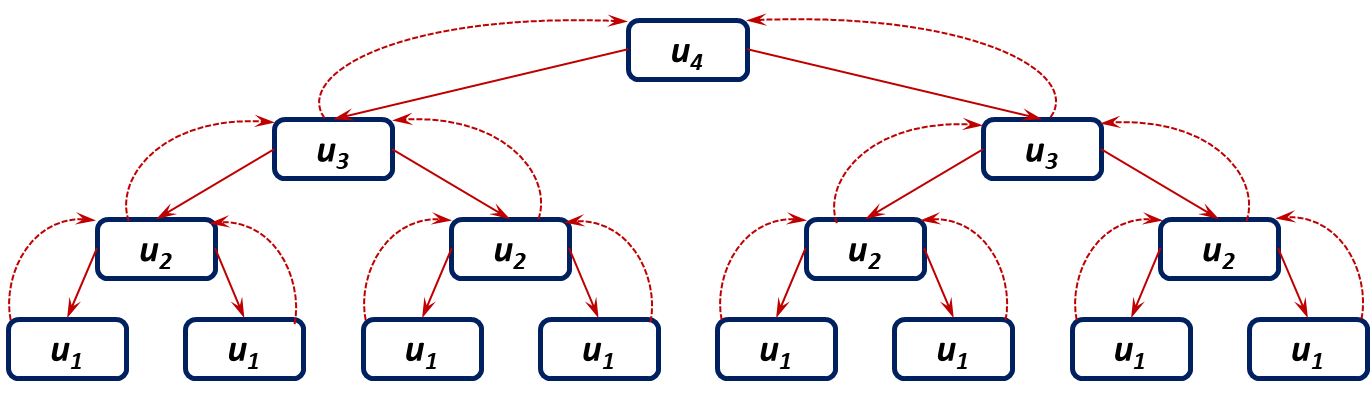
\includegraphics[width=3cm]{fig_01}\\
%\textit{}
}%figues de la page de garde

\def\xxtitreexo{Applications -- Bases}
\def\xxsourceexo{}
\def\xxactivite{{ Application 02} \ifprof  -- Corrigé \else \fi}

%\iflivret
\input{\repRel/Style/pagegarde_TD}
%\else
%\pagestyle{empty}


%%%%%%%% PAGE DE GARDE COURS
\ifcours
\begin{tikzpicture}[remember picture,overlay]
\node at (current page.north west)
{\begin{tikzpicture}[remember picture,overlay]
\node[anchor=north west,inner sep=0pt] at (0,0) {\includegraphics[width=\paperwidth]{\thechapterimage}};
\draw[anchor=west] (-2cm,-8cm) node [line width=2pt,rounded corners=15pt,draw=ocre,fill=white,fill opacity=0.6,inner sep=40pt]{\strut\makebox[22cm]{}};
\draw[anchor=west] (1cm,-8cm) node {\huge\sffamily\bfseries\color{black} %
\begin{minipage}{1cm}
\rotatebox{90}{\LARGE\sffamily\textsc{\color{ocre}\textbf{\xxnumpartie}}}
\end{minipage} \hfill
\begin{minipage}[c]{14cm}
\begin{titrepartie}
\begin{flushright}
\renewcommand{\baselinestretch}{1.1} 
\Large\sffamily\textsc{\textbf{\xxpartie}}
\renewcommand{\baselinestretch}{1} 
\end{flushright}
\end{titrepartie}
\end{minipage} \hfill
\begin{minipage}[c]{3.5cm}
{\large\sffamily\textsc{\textbf{\color{ocre} \discipline}}}
\end{minipage} 
 };
\end{tikzpicture}};
\end{tikzpicture}


\begin{tikzpicture}[overlay]
\node[shape=rectangle, 
      rounded corners = .25 cm,
	  draw= ocre,
	  line width=2pt, 
	  fill = ocre!10,
	  minimum width  = 2.5cm,
	  minimum height = 3cm,] at (18cm,0) {};
\node at (17.7cm,0) {\rotatebox{90}{\textbf{\Large\color{ocre}{\classe}}}};
%{};
\end{tikzpicture}

\vspace{3.5cm}

\begin{tikzpicture}[remember picture,overlay]
\draw[anchor=west] (-2cm,-6cm) node {\huge\sffamily\bfseries\color{black} %
\begin{minipage}{2cm}
\begin{center}
\LARGE\sffamily\textsc{\color{ocre}\textbf{\xxactivite}}
\end{center}
\end{minipage} \hfill
\begin{minipage}[c]{15cm}
\begin{titrechapitre}
\renewcommand{\baselinestretch}{1.1} 
\Large\sffamily\textsc{\textbf{\xxnumchapitre}}

\Large\sffamily\textsc{\textbf{\xxchapitre}}
\vspace{.5cm}

\renewcommand{\baselinestretch}{1} 
\normalsize\normalfont
\xxcompetences
\end{titrechapitre}
\end{minipage}  };
\end{tikzpicture}
\vfill

\begin{flushright}
\begin{minipage}[c]{.3\linewidth}
\begin{center}
\xxfigures
\end{center}
\end{minipage}\hfill
\begin{minipage}[c]{.6\linewidth}
\startcontents
\printcontents{}{1}{}
\end{minipage}
\end{flushright}

\begin{tikzpicture}[remember picture,overlay]
\draw[anchor=west] (4.5cm,-.7cm) node {
\begin{minipage}[c]{.2\linewidth}
\begin{flushright}

\includegraphics[width=2cm]{png/logoCC}
\end{flushright}
\end{minipage}
\begin{minipage}[c]{.2\linewidth}
\textsl{\xxauteur} \\
\textsl{\classe}
\end{minipage}
 };
\end{tikzpicture}
\newpage
\pagestyle{fancy}

\newpage
\pagestyle{fancy}

\else
\fi


%%%%%%%% PAGE DE GARDE TD
\iftd
%\begin{tikzpicture}[remember picture,overlay]
%\node at (current page.north west)
%{\begin{tikzpicture}[remember picture,overlay]
%\draw[anchor=west] (-2cm,-3.25cm) node [line width=2pt,rounded corners=15pt,draw=ocre,fill=white,fill opacity=0.6,inner sep=40pt]{\strut\makebox[22cm]{}};
%\draw[anchor=west] (1cm,-3.25cm) node {\huge\sffamily\bfseries\color{black} %
%\begin{minipage}{1cm}
%\rotatebox{90}{\LARGE\sffamily\textsc{\color{ocre}\textbf{\xxnumpartie}}}
%\end{minipage} \hfill
%\begin{minipage}[c]{13.5cm}
%\begin{titrepartie}
%\begin{flushright}
%\renewcommand{\baselinestretch}{1.1} 
%\Large\sffamily\textsc{\textbf{\xxpartie}}
%\renewcommand{\baselinestretch}{1} 
%\end{flushright}
%\end{titrepartie}
%\end{minipage} \hfill
%\begin{minipage}[c]{3.5cm}
%{\large\sffamily\textsc{\textbf{\color{ocre} \discipline}}}
%\end{minipage} 
% };
%\end{tikzpicture}};
%\end{tikzpicture}

%%%%%%%%%% PAGE DE GARDE TD %%%%%%%%%%%%%%%
%\begin{tikzpicture}[overlay]
%\node[shape=rectangle, 
%      rounded corners = .25 cm,
%	  draw= ocre,
%	  line width=2pt, 
%	  fill = ocre!10,
%	  minimum width  = 2.5cm,
%	  minimum height = 2.5cm,] at (18.5cm,0) {};
%\node at (17.7cm,0) {\rotatebox{90}{\textbf{\Large\color{ocre}{\classe}}}};
%%{};
%\end{tikzpicture}

% PARTIE ET CHAPITRE
%\begin{tikzpicture}[remember picture,overlay]
%\draw[anchor=west] (-1cm,-2.1cm) node {\large\sffamily\bfseries\color{black} %
%\begin{minipage}[c]{15cm}
%\begin{flushleft}
%\xxnumchapitre \\
%\xxchapitre
%\end{flushleft}
%\end{minipage}  };
%\end{tikzpicture}

% Bandeau titre exo
\begin{tikzpicture}[remember picture,overlay]
\draw[anchor=west] (-2cm,-4cm) node {\huge\sffamily\bfseries\color{black} %
\begin{minipage}{5cm}
\begin{center}
\LARGE\sffamily\color{ocre}\textbf{\textsc{\xxactivite}}

\begin{center}
\xxfigures
\end{center}

\end{center}
\end{minipage} \hfill
\begin{minipage}[c]{12cm}
\begin{titrechapitre}
\renewcommand{\baselinestretch}{1.1} 
\large\sffamily\textbf{\textsc{\xxtitreexo}}

\small\sffamily{\textbf{\textit{\color{black!70}\xxsourceexo}}}
\vspace{.5cm}

\renewcommand{\baselinestretch}{1} 
\normalsize\normalfont
\xxcompetences
\end{titrechapitre}
\end{minipage}  };
\end{tikzpicture}
\else
\fi


%%%%%%%% PAGE DE GARDE FICHE
\iffiche
\begin{tikzpicture}[remember picture,overlay]
\node at (current page.north west)
{\begin{tikzpicture}[remember picture,overlay]
\draw[anchor=west] (-2cm,-3.25cm) node [line width=2pt,rounded corners=15pt,draw=ocre,fill=white,fill opacity=0.6,inner sep=40pt]{\strut\makebox[22cm]{}};
\draw[anchor=west] (1cm,-3.25cm) node {\huge\sffamily\bfseries\color{black} %
\begin{minipage}{1cm}
\rotatebox{90}{\LARGE\sffamily\textsc{\color{ocre}\textbf{\xxnumpartie}}}
\end{minipage} \hfill
\begin{minipage}[c]{14cm}
\begin{titrepartie}
\begin{flushright}
\renewcommand{\baselinestretch}{1.1} 
\large\sffamily\textsc{\textbf{\xxpartie} \\} 

\vspace{.2cm}

\normalsize\sffamily\textsc{\textbf{\xxnumchapitre -- \xxchapitre}}
\renewcommand{\baselinestretch}{1} 
\end{flushright}
\end{titrepartie}
\end{minipage} \hfill
\begin{minipage}[c]{3.5cm}
{\large\sffamily\textsc{\textbf{\color{ocre} \discipline}}}
\end{minipage} 
 };
\end{tikzpicture}};
\end{tikzpicture}


\begin{tikzpicture}[overlay]
\node[shape=rectangle, 
      rounded corners = .25 cm,
	  draw= ocre,
	  line width=2pt, 
	  fill = ocre!10,
	  minimum width  = 2.5cm,
	  minimum height = 2.5cm,] at (18.5cm,0.5cm) {};
%	  minimum height = 2.5cm,] at (18.5cm,0cm) {};
\node at (17.7cm,0.5) {\rotatebox{90}{\textsf{\textbf{\large\color{ocre}{\classe}}}}};
%{};
\end{tikzpicture}

\else
\fi



%\fi

\setlength{\columnseprule}{.1pt}

\pagestyle{fancy}
\thispagestyle{plain}


\vspace{4.5cm}

\def\columnseprulecolor{\color{bleuxp}}
\setlength{\columnseprule}{0.4pt} 







\ifprof
\vspace{1cm}
\else
\begin{multicols}{2}
\fi


\section*{Prise en main en mode << exécution d'un fichier >>}
\textbf{Lancer Pyzo}

Pour écrire de véritables programmes et les conserver, il faut créer un fichier lstlisting exécutable, ce qu'on appelle aussi un "script".\\ 
Pour cela, à partir de l'interpréteur : 
\begin{center} \fbox{aller dans "File" et cliquer sur "New"}
\end{center} (plus rapide : \fbox{CTRL}+\fbox{N}).\\

Avant toute chose, enregistrer ce fichier dans votre répertoire "TP0" sous le nom TP0.py ; il ne faut pas oublier de préciser  l'extension .py ("File" puis "Save" ou \fbox{CTRL}+\fbox{S}).\\


Taper dans le fichier les lignes suivantes : 
\begin{lstlisting}
2 * 3
print(3 * 3)
a = 4 * 3
print(a + 2)
\end{lstlisting}
Sauvegarder, puis \textbf{exécuter} (\textit{run} en anglais) 
\begin{center} 
\fbox{en tapant \fbox{CTRL}+\fbox{E}}
\fbox{ou en cliquant sur "Execute file" dans le menu "Run"}
\end{center}

Si votre script fait appel à des fichiers stockés dans le même dossier que votre script, la première exécution doit repérer le chemin d'accès aux données, dans ce cas là, exécuter :
\begin{center} 
\textbf{en cliquant droit sur l'onglet de votre script et en sélectionnant "Run file as script".}
\end{center}
\question{Commenter}
\ifprof
\begin{corrige}
Seul le résultat de 3*5 et de a+2 s'est affiché. Les autres calculs ou affectations ont bien été effectués mais non affichés. En mode "exécution de fichier", on peut donc choisir ce qu'on affiche.
\end{corrige}
\else
\fi

\exer{}

\question{Créez dans votre script deux variables \texttt{x} et \texttt{y} contenant des entiers de votre choix. }
\begin{enumerate}
\item Complétez votre script pour qu'à l'exécution,  il s'affiche dans le shell le booléen disant si \texttt{x} est pair ou non.
\item Complétez votre script pour qu'à l'exécution,  il s'affiche dans le shell le booléen disant si \texttt{x} et \texttt{y} sont de même parité ou non.
\end{enumerate}


\exer{}

\question{Créez dans votre script deux variables \texttt{prenom} et \texttt{nom} de type chaîne de caractère. }
\question{ Complétez votre script pour qu'à l'exécution,  il s'affiche vos initiales (par exemple \texttt{LM} pour Léa Martin).}


Après ce premier test et ces deux exercices, votre script ressemble à peu près à cela : 
\begin{lstlisting}
2 * 3
print(3 * 3)
a = 4 * 3
print(a + 2)
x = 2
y  = 5
###
# ce que vous avez répondu pour l'exo précédent 
###
prenom = 'Léa'\\
nom = 'Martin'\\

###
# ce que vous avez répondu pour cet exercice.
###
\end{lstlisting}
Ainsi, on ne voit pas bien la délimitation des différents exercices ; de plus, lorsqu'on exécute ce script, on a les affichages "parasites" du test et de tous les exercices, alors qu'on aimerait passer à autre chose...Il ne faut pas effacer votre travail pour autant !\\
Il convient donc d'utiliser des \textbf{commentaires} à l'aide du symbole \# ; tout ce qui suit sur la même ligne ne sera pas "lu". On s'en sert pour améliorer la présentation, et pour supprimer les affichages intempestifs lors de l'exécution. Par exemple, il convient de transformer notre fichier ainsi : 

\begin{lstlisting}
##### TP 0 Prise en main de Python #####
## Premier test

2 * 5           
#print(3 * 5) 
a = 4 * 5 \\
#print(a + 2) 

## Exercice 4
x = 2
y = 5 
# ...ce que vous avez répondu pour l'exo 4, que vous pouvez mettre en commentaire !

## Exercice  5\\
prenom = 'Léa'\\
nom = 'Martin'\\
# ...ce que vous avez répondu pour l'exo 5, que vous pouvez mettre en commentaire !
\end{lstlisting}

On peut mettre tout un paragraphe en commentaire en le sélectionnant, puis en allant dans le menu "Format" et en cliquant sur "Comment Out Region". L'opération inverse se fait avec "Uncomment Region".\\


Lorsqu'on ferme PYZO et qu'on le relance, votre fichier TP0.py se retrouvera facilement en cliquant sur "Open" dans le menu "File", ou bien en faisant \fbox{CTRL}+\fbox{O}.

\exer{}

\question{Toujours en se servant des variables \texttt{prenom} et \texttt{nom}, écrire les instructions permettant d'afficher par exemple le message : \texttt{'Bonjour, Léa Martin !'} lorsque \texttt{prenom} contient \texttt{'Léa'} et \texttt{nom} contient \texttt{'Martin'}.}








\ifprof
\else
\end{multicols}
\fi

